\documentclass{article}
\usepackage[hyphens]{url}
\usepackage{mathtools}
\usepackage{amsmath}
\usepackage{listings}
\usepackage{graphicx}
\usepackage[margin=1in]{geometry}
\usepackage{float}
\floatstyle{boxed}
\restylefloat{figure}
\lstset{basicstyle=\footnotesize, breaklines=true}
\begin{document}


\title{CS595 Intro to Web Science, Assignment \#7}
\author{Valentina Neblitt-Jones}
\date{November 7, 2013}
\maketitle



\section*{Question 1}

Using D3, create a graph of the Karate club before and after the split \\

Weight the edges with data from: \url{http://vlado.fmf.uni-lj.si/pub/networks/data/ucinet/zachary.dat} \\

Have the transition from before/after the split occur on a mouse click.  \\

%\begin{itemize}
%\item 
%\item
%\end{itemize}

\subsection*{Answer to Question 1}

To begin, I needed to get zachary.dat into a JSON format so I needed a dictionary with two lists inside. i read in each line - skipping the header data and the matrix showing mere connections - of the dat file and assigned it to person. Then I looped through the lines to create the ``name'' (we did not have their names so numbers were used). An second loop was needed in order to go through each line and access the weight.  I needed to ignore the weights that equaled zero so only the weights of 1 or higher were included. I did not exclude the duplicate pairings (e.g. 1, 32, 4 and 32, 1, 4). My guess is that the duplicates would not cause a problem, but I remain unsure. I then used json.dumps to output the data in the JSON format. (Listing \ref{code1})


\begin{lstlisting}[frame=single, caption=CreateJSONFile01.py, label=code1]
import json
import pprint

g = open('zachary1.json', 'w')
pp = pprint.PrettyPrinter()

adict = {}
adict["nodes"] = []
adict["links"] = []

id = 0 # name

with open('zachary.dat', 'r') as f:
   good = f.readlines()[41:]
for line in good:
	person = line.split()
	id = id + 1 # generates name
	adict["nodes"].append({'id':str(id)})
	for i in range(0, len(person)):
		weight = int(person[i])
		source = id - 1
		target = i
		if weight != 0:
			adict["links"].append({'source': source, 'target': target, 'weight':weight})
			
pp.pprint(adict)
output = json.dumps(adict, indent=4)
g.write(output)

f.close()
g.close()\end{lstlisting}

The next step was to use the JSON file from the previous step in order to create the graph of the club after the split. I opened the file using json.load and used node\_link\_graph to turn the input into something that networkX could work with. In the previous assignment, we did something similar, but I implemented it in R so I needed to translate the steps from R to Python. Because we were emulating the group splitting into two groups, the while looped kept functioning until the number of connected components reached 2. First, I calculated the edge betweenness. Then I looped through the edge betweenness values while keeping track of the max edge betweenness value. Finally, it deleted the edge for the highest value until the connected components was equal to 2. Next, the result was converted back to data with node\_link\_data and outputted as JSON with json.dumps. (Listing \ref{code2})

\begin{lstlisting}[frame=single, caption=CreateJSONFile02.py, label=code2]
import json
import pprint
import networkx
from networkx.readwrite import json_graph

pp = pprint.PrettyPrinter()

f = open('zachary1.json')
g = open('zachary2.json', 'w')

data = json.load(f)
# pp.pprint(data)
f.close()

G = json_graph.node_link_graph(data)

while networkx.number_connected_components(G) < 2:
	edgy = networkx.edge_betweenness_centrality(G)
	maxb = 0
	for edge in edgy:
		#print('key ' + str(edge) + ' value ' + str(edgy[edge]))
		if edgy[edge] > maxb:
			maxb = edgy[edge]
			maxedge = edge

	G.remove_edge(maxedge[0],maxedge[1])

result = json_graph.node_link_data(G)

g.write(json.dumps(result, indent=4))
g.close()
\end{lstlisting}

I followed an example in Scott Murray's book \emph {Interactive Data Visualization}, which is how I ended up with the colorful unlabeled circles. He covered how to make one graph, but not how to do the transformation from one to the other on mouse click. So looking at Listing \ref{webpage}, I changed the height and width because the graphs would need more room in order to show the split. I added a transformation attribute to create the call for transformation. I load the original graph first. The transforming function needed to remove the original graph's elements before loading the new elements. The elements of the code that were true for both graphs are contained within d3.json(jsonfile, function(error, dataset). I adjusted force.gravity to a lower number since the split was not clear. The split components were initially still too close to each other to see that they had actually split apart. I followed the Bostock example at \url{http://bl.ocks.org/mbostock/950642} to add the labels to the colorful nodes. Figure \ref{before} shows the club before the split and Figure \ref{after} shows the club after the split. The animation demonstration can be found at \url{http://www.cs.odu.edu/~vneblitt/cs595/}.


\begin{lstlisting}[frame=single, caption=index.html, label=webpage]
<script type="text/javascript">

//Width and height
var w = 900;
var h = 900;
                        
//Create SVG element
var svg = d3.select("body")
	.append("svg")
	.attr("width", w)
	.attr("height", h)
	.on("click", transformit);
                            
loadjson('zachary1.json');
                            
function transformit() {
	d3.selectAll("line").remove();
	d3.selectAll(".node").remove();
	loadjson('zachary2.json');                        
	}

function loadjson(jsonfile) {
                        
d3.json(jsonfile, function(error, dataset) {
                        
//Initialize a default force layout, using the nodes and edges in dataset
var force = d3.layout.force()
	.nodes(dataset.nodes)
	.links(dataset.links)
	.size([w, h])
	.linkDistance(100)
	.charge(-100)
	.gravity(0.05)
	.start();

var colors = d3.scale.category10();
                        
//Create edges as lines
var links = svg.selectAll("line")
	.data(dataset.links)
	.enter()
	.append("line")
	.style("stroke", "#ccc")
	.style("stroke-width", 1);
                        
//Create nodes as circles
var node = svg.selectAll(".node")
	.data(dataset.nodes)
	.enter().append("g")
	.attr("class", "node")
	.call(force.drag);

node.append("circle")
	.style("fill", function(d, i) {
		return colors(i);
	})
	.attr("cx", -8)
	.attr("cy", -8)
	.attr("r", 10);

node.append("text")
.attr("dx", 12)
.attr("dy", ".35em")
.text(function(d) { return d.id });
                            
 //Every time the simulation "ticks", this will be called
force.on("tick", function() {
links.attr("x1", function(d) { return d.source.x; })
	.attr("y1", function(d) { return d.source.y; })
	.attr("x2", function(d) { return d.target.x; })
	.attr("y2", function(d) { return d.target.y; });
                        
node.attr("transform", function(d) { return "translate(" + d.x + "," + d.y + ")"; });
        
 	});
                        
});
                        
}
 </script>
 \end{lstlisting}

\begin{figure}[H]
\centering
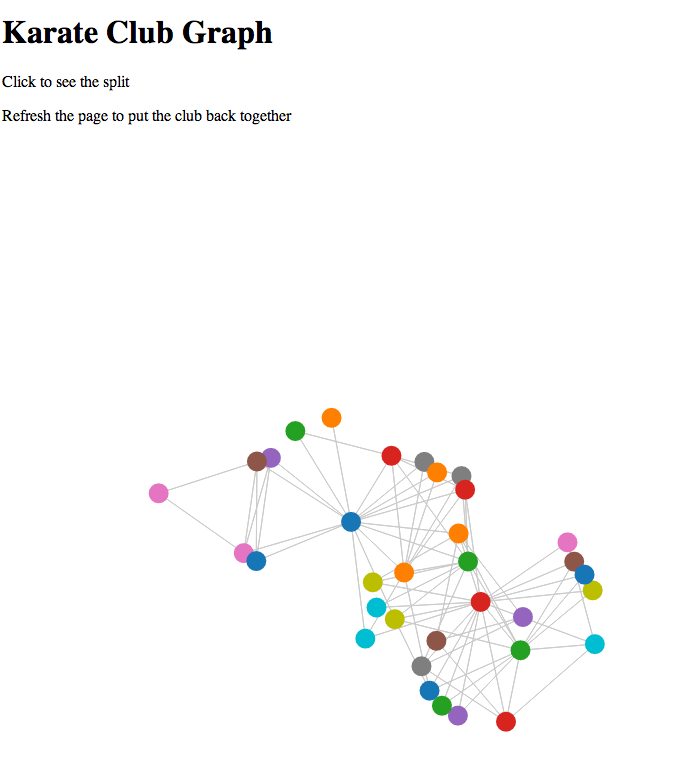
\includegraphics[scale=0.50]{q1/kcbeforesplit}
\caption{Karate Club Before Split}
\label{before}
\end{figure}

\begin{figure}[H]
\centering
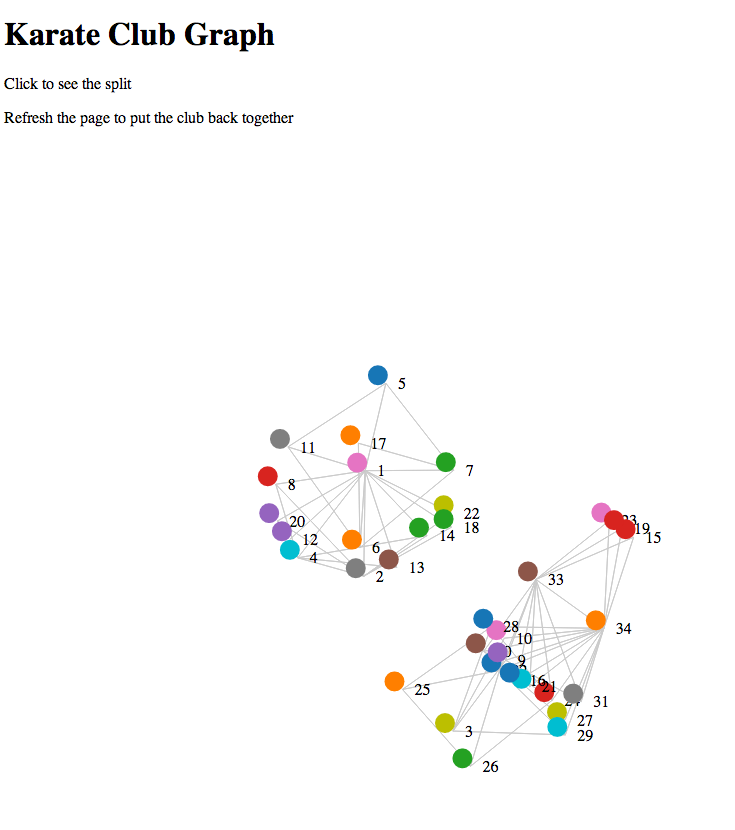
\includegraphics[scale=0.50]{q1/kcaftersplit}
\caption{Karate Club After Split}
\label{after}
\end{figure}

%\begin{figure}[H]
%\centering
%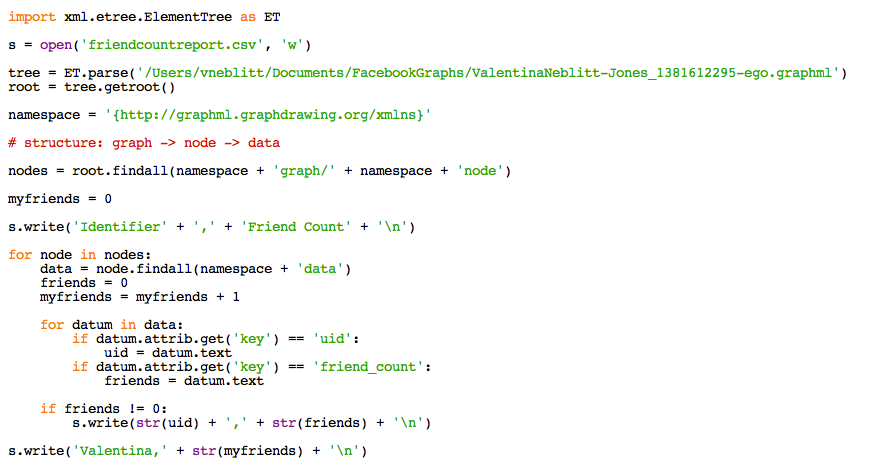
\includegraphics[scale=0.50]{q1/GetFriendCountsCode}
%\caption{Showing Friend Count}
%\label{GetFriendCountsCode}
%\end{figure}

%\begin{table}[!h]
%\centering

%\begin{tabular}{c c c c}
%\hline
%Identifier & Model &  Actual & Hit/Miss \\
%\hline
%\hline
%1 & Mr. Hi & Mr. Hi & Hit \\
%2 & Mr. Hi & Mr. Hi & Hit \\
%3 & Mr. Hi & Mr. Hi & Hit \\
%4 & Mr. Hi & Mr. Hi & Hit \\
%5 & Mr. Hi & Mr. Hi & Hit \\
%6 & Mr. Hi & Mr. Hi & Hit \\
%7 & Mr. Hi & Mr. Hi & Hit \\
%8 & Mr. Hi & Mr. Hi & Hit \\
%9 & Mr. Hi & Mr. Hi & Hit \\
%10 & Mr. Hi & John & Miss \\
%\hline
%\end{tabular}
%\caption{Results of Model vs. Actual}
%\end{table}

\newpage

\section*{Extra Credit, 3 Points}

Use D3 to create a who-follows-whom graph of your Twitter account. Use my Twitter account (phonedude\_mln) if you do not have an interesting number of followers.

%\begin{table}[!h]
%\centering
%\caption{Results of Model vs. Actual}
%\begin{tabular}{c c c c}
%\hline
%Identifier & Model &  Actual & Hit/Miss \\
%\hline
%\hline
%0.150 & 0.014 & Mr. Hi & Hit \\
%0.085 & John & Mr. Hi & Hit \\
%\hline
%\end{tabular}
%\end{table}

\subsection*{Answer to Extra Credit}

Not attempted.



\newpage

\section*{Resources}

Note: Apologies. I did not have time to implement BibTex for this assignment, but I will on Assignments 8, 9, and 10.

\begin{itemize}
\item Bostock, Michael. Data-Driven Documents. \url{http://d3js.org/}
\item Bostock, Michael. Labeled Force Layout. \url{http://bl.ocks.org/mbostock/950642}
\item Bostock, Michael. Selections. \url{https://github.com/mbostock/d3/wiki/Selections#wiki-on}
\item Bostock, Michael. mbostock/d3. \url{https://github.com/mbostock/d3}
\item Bostock, Michael. mbostock/d3: API Reference. \url{https://github.com/mbostock/d3/wiki/API-Reference}
\item Murray, Scott. About these tutorial. \url{http://alignedleft.com/tutorials/d3/about}
\item Murray, Scott. Interactive Data Visualization: An Introduction to Designing with D3. Via Safari Books Online
\item NetworkX developer team. NetworkX. \url{http://networkx.github.io/}
\item NetworkX developer team. NetworkX: edge\_betweenness\_centrality. \url{http://networkx.github.io/documentation/latest/reference/generated/networkx.algorithms.centrality.edge_betweenness_centrality.html#networkx.algorithms.centrality.edge_betweenness_centrality}
\item NetworkX developer team. NetworkX: Graph - Undirected graphs with self loops. \url{http://networkx.github.io/documentation/latest/reference/classes.graph.html#networkx.Graph}
\item NetworkX developer team. NetworkX: node\_link\_data. \url{http://networkx.lanl.gov/reference/generated/networkx.readwrite.json_graph.node_link_data.html#networkx.readwrite.json_graph.node_link_data}
\item NetworkX developer team. NetworkX: node\_link\_graph. \url{http://networkx.lanl.gov/reference/generated/networkx.readwrite.json_graph.node_link_graph.html#networkx.readwrite.json_graph.node_link_graph}
\item NetworkX developer team. NetworkX: number\_connected\_components. \url{http://networkx.github.io/documentation/latest/reference/generated/networkx.algorithms.components.connected.number_connected_components.html#networkx.algorithms.components.connected.number_connected_components}
\item PyMOTW. json: JavaScript Objection Notation Serializer. \url{http://pymotw.com/2/json/}
\item Python.org. json: JSON encoder and decoder. \url{http://docs.python.org/3.3/library/json.html}
\item Python.org. print: Data pretty printer. \url{http://docs.python.org/2/library/pprint.html}
\item Stack Overflow. Parsing values from a JSON file in Python. \url{http://stackoverflow.com/questions/2835559/parsing-values-from-a-json-file-in-python}
\item Stack Overflow. Skip the first couple of lines while reading lines in Python file. \url{http://stackoverflow.com/questions/9578580/skip-first-couple-of-lines-while-reading-lines-in-python-file}



\end{itemize}

\end{document}